\documentclass{scrartcl}
\usepackage[utf8]{inputenc}
%\usepackage[T1]{fontenc}
\usepackage[a4paper, left=2.5cm, right=2.5cm, top=2.5cm, bottom=4cm]{geometry}
\usepackage[english]{babel}
\usepackage{amsmath, amsthm, amssymb, amstext}
\usepackage{listings}
\usepackage{color}
\usepackage{graphicx}
\usepackage{xparse}
\usepackage{fancyhdr}
\usepackage{algorithmicx}
\usepackage{algpseudocode}
\usepackage{algorithm}
\usepackage{parskip}
\usepackage[table]{xcolor}
\usepackage{tabularx}
\usepackage{enumerate}
\usepackage{enumitem}
\usepackage{float}
%\usepackage{minted}
\usepackage {tikz}
\usetikzlibrary{positioning}
\usepackage{marvosym}

\pagestyle{fancy}


\rhead{{\newcommand\and\\\getauthors}}
\author{Felix Bühler\\2973410 \and Clemens Lieb\\3130838 \and Steffen Wonner\\2862123 \and Fabian Bühler\\2953320}
\lhead{\textbf\gettitle}
\title{\gettitle}
\chead{\getsubtitle}
\subtitle{\getsubtitle}

\addtolength{\headheight}{2\baselineskip}
\renewcommand{\headrulewidth}{0pt}

\newcommand{\gettitle}{Distributed systems I\\Winter Term 2019/20}
\newcommand{\getsubtitle}{G2T1 – Assignment 6 (theoretical part)}
\newcommand{\getauthors}{Felix Bühler \and Clemens Lieb \and Steffen Wonner \and Fabian Bühler}
\setlength{\headheight}{53pt}

\begin{document}
\maketitle

\section*{1 - Replication with Atomic Multicast}

\section*{2 - Multicast Semantics}

\section*{3 - Causal Mulitcast}

\subsection*{a)}
\subsubsection*{i.}
See figure \ref{fig:3a}

\begin{figure}[!ht]
	\centering
	\begin{tikzpicture}
	\draw[->, thick] (0, 6) -- (12, 6);
	\draw[->, thick] (0, 3) -- (12, 3);
	\draw[->, thick] (0, 0) -- (12, 0);
	
	\foreach \t/\p in {1/6,2/3,3/0} {
		\draw node at (-0.5, \p) {\(P_\t\)};
	};

	\draw[->, thick] (0.5, 6) -- node[pos=0.1, right] {$ m_1 $} (6, 0);
	\draw[->, thick] (0.5, 6) -- (1, 3);
	
	\draw[->, thick] (2.5, 3) -- (5, 6);
	\draw[->, thick] (2.5, 3) -- node[pos=0.3, left] {$ m_2 $} (4, 0);
	\draw[->, blue, thick] (4, 0) to [out=30,in=150] (7, 0);
	
	\draw[->, thick] (6.5, 3) -- node[pos=0.3, left] {$ m_3 $} (11, 6);
	\draw[->, thick] (6.5, 3) -- (10, 0);
	
	\draw[->, thick] (8, 0) -- (9.5, 3);
	\draw[->, thick] (8, 0) -- node[pos=0.1, left] {$ m_4 $} (9.5, 6);
		
	\draw node at (0.5, 6.3) {$ [1,0,0] $};
	\draw node at (5, 6.3) {$ [1,1,0] $};
	\draw node at (9.5, 6.3) {$ [1,1,1] $};
	\draw node at (11, 6.3) {$ [1,2,1] $};
	
	\draw node at (1, 2.7) {$ [1,0,0] $};
	\draw node at (2, 3.3) {$ [1,1,0] $};
	\draw node at (6, 3.3) {$ [1,2,0] $};
	\draw node at (9.5, 3.3) {$ [1,2,1] $};
	
	\draw node at (4, -0.3) {$ [1,1,0] $};
	\draw node[green] at (6, -0.3) {$ [1,1,0] $};
	\draw node[blue] at (7, 0.3) {$ [1,1,0] $};
	\draw node at (8, -0.3) {$ [1,1,1] $};
	\draw node at (10, -0.3) {$ [1,2,1] $};
	
	\end{tikzpicture}
	\caption{Execution of CBCAST Algorith}
	\label{fig:3a}
\end{figure}

\subsubsection*{ii.}

The delivered message $ m_2 $ on $ P_3 $ has to be delayed. The \textcolor{green}{green} VectorClock would be $ [1,0,0] $ and the \textcolor{blue}{blue} $ m_2 $ message would be delayed, so the vector clock would be updated to $ [1,1,0] $ after the recieved $ m_1 $ message.

\subsection*{b)}
\subsubsection*{i.}
\subsubsection*{ii.}
\subsubsection*{iii.}

\end{document}
